\documentclass[11pt,letterpaper]{article}

\usepackage[margin=0.90in,top=0.92in,bottom=0.92in]{geometry}
\usepackage[utf8]{inputenc}
\usepackage[T1]{fontenc}
\usepackage{newpxtext,newpxmath} % Palatino typography
\usepackage{microtype}
\usepackage{amsmath,amsfonts}
\usepackage{graphicx}
\usepackage{booktabs}
\usepackage{xcolor}
\usepackage{fancyhdr}
\usepackage{enumitem}
\usepackage{titlesec}
\usepackage{tikz}
\usetikzlibrary{shapes.geometric,arrows.meta,positioning,calc,decorations.pathmorphing}
\usepackage{listings}
\usepackage{hyperref}

% Palette
\definecolor{primaryblue}{RGB}{2, 100, 160}
\definecolor{accentindigo}{RGB}{60, 50, 190}
\definecolor{accentteal}{RGB}{12, 110, 105}
\definecolor{darkslate}{RGB}{28, 38, 52}
\definecolor{warmbg}{RGB}{252, 250, 247}
\definecolor{boxborder}{RGB}{210, 220, 230}
\definecolor{calloutbg}{RGB}{242, 248, 255}
\definecolor{codebg}{RGB}{247, 249, 252}
\definecolor{codeframe}{RGB}{220, 228, 238}

% Hyperref
\hypersetup{
    colorlinks=true,
    linkcolor=accentindigo,
    citecolor=primaryblue,
    urlcolor=accentteal
}

% Section Titles - Concise, colon-free
\titleformat{\section}{\Large\bfseries\color{primaryblue}}{\thesection.}{0.6em}{}[\vspace{-0.3em}{\color{boxborder}\hrule height 0.7pt}]
\titleformat{\subsection}{\large\bfseries\color{accentindigo}}{\thesubsection}{0.6em}{}
\titleformat{\subsubsection}{\normalsize\bfseries\color{darkslate}}{\thesubsubsection}{0.6em}{}
\titlespacing*{\section}{0pt}{5pt plus 1.5pt minus 1pt}{2.5pt plus 1pt minus 1pt}
\titlespacing*{\subsection}{0pt}{3.5pt plus 1pt minus 1pt}{1.5pt plus 1pt minus 1pt}
\setlength{\abovedisplayskip}{3.5pt plus 1pt minus 1pt}
\setlength{\belowdisplayskip}{3.5pt plus 1pt minus 1pt}
\setlength{\abovedisplayshortskip}{2pt plus 1pt minus 1pt}
\setlength{\belowdisplayshortskip}{2pt plus 1pt minus 1pt}

% Headers / Footers
\pagestyle{fancy}
\fancyhf{}
\fancyhead[L]{\small\sffamily\color{darkslate}\textbf{Cultural Mechanics}}
\fancyhead[R]{\small\sffamily\color{primaryblue}\textbf{Lecture 04}}
\fancyfoot[L]{\scriptsize\sffamily\color{darkslate!60}Semantic Mechanics Project $\cdot$ Mathematical Linguistics Group}
\fancyfoot[R]{\small\sffamily\color{darkslate}\thepage}
\renewcommand{\headrulewidth}{0.4pt}
\renewcommand{\footrulewidth}{0.4pt}

% Callout Boxes
\newcommand{\calloutbox}[2]{%
\vspace{0.35em}\noindent
\begin{tikzpicture}
\node[draw=primaryblue, fill=calloutbg, rounded corners=4pt, line width=0.9pt, text width=\dimexpr\linewidth-24pt\relax, inner sep=7.5pt] {
    {\sffamily\bfseries\color{primaryblue}#1}\par\vspace{0.25em}{\color{boxborder}\hrule height 0.5pt}\vspace{0.45em}
    {\small\color{darkslate}#2}
};
\end{tikzpicture}\vspace{0.35em}
}

\newcommand{\socraticbox}[2]{%
\vspace{0.35em}\noindent
\begin{tikzpicture}
\node[draw=accentindigo, fill=warmbg, rounded corners=4pt, line width=0.9pt, text width=\dimexpr\linewidth-24pt\relax, inner sep=7.5pt] {
    {\sffamily\bfseries\color{accentindigo}#1}\par\vspace{0.25em}{\color{boxborder}\hrule height 0.5pt}\vspace{0.45em}
    {\small\color{darkslate}#2}
};
\end{tikzpicture}\vspace{0.35em}
}

% Code Listings Configuration
\lstset{
    backgroundcolor=\color{codebg},
    frame=single,
    rulecolor=\color{codeframe},
    basicstyle=\ttfamily\footnotesize\color{darkslate},
    keywordstyle=\bfseries\color{accentindigo},
    commentstyle=\itshape\color{accentteal},
    stringstyle=\color{primaryblue},
    breaklines=true,
    tabsize=4,
    showstringspaces=false,
    captionpos=b,
    xleftmargin=6pt,
    xrightmargin=6pt
}

% Float Spacing
\setlength{\textfloatsep}{7pt plus 2pt minus 2pt}
\setlength{\intextsep}{5pt plus 2pt minus 2pt}
\setlength{\abovecaptionskip}{3.5pt}
\setlength{\belowcaptionskip}{3.5pt}

\begin{document}

% Title Block
\begin{center}
    {\small\sffamily\bfseries\color{darkslate} SEMANTIC MECHANICS PROJECT $\cdot$ MATHEMATICAL LINGUISTICS GROUP}\\[0.7em]
    {\LARGE\bfseries\color{primaryblue} Lecture 04: Thermodynamic Semiotics}\\[0.35em]
    {\Large\bfseries\color{primaryblue} The Physics of Sequence Transformation and Typographic Work}\\[0.4em]
    {\normalsize\sffamily\color{darkslate} \textbf{Course:} Cultural Mechanics $\cdot$ \textbf{Semester:} Autumn 2026}\\[0.25em]
    {\small\sffamily\color{darkslate!80} \textbf{Prerequisites:} Statistical Mechanics, Information Theory, Algorithmic Complexity, Linear Algebra}\\[0.25em]
    {\small\sffamily\color{darkslate!80} \textbf{Foundational Readings:} Landauer (1961), Bennett (1973), Shannon (1948), Kolmogorov (1965), Bringhurst (1992)}
\end{center}
\vspace{0.1em}
\hrule height 1.2pt \vspace{0.7em}

\section{Thermodynamic Foundations of Semiosis}

Welcome to \textit{Lecture 04: Thermodynamic Semiotics}. In Lecture 03, we formalized the differential geometry and category-theoretic invariants of translation, establishing that cross-lingual transfer maps continuous manifolds via smooth pushforwards and adjoint functors. Yet every physical intelligence system---from human scribes pressing reeds into wet Sumerian clay to GPU clusters executing billion-parameter matrix products---is fundamentally a \textbf{non-equilibrium thermodynamic engine} constrained by the physical laws of matter, energy, and entropy dissipation.

Symbols are never disembodied abstractions. A sign is an ordered physical configuration of matter and energy: ink pigments bonded to cellulose fibers, crystalline domain orientations on magnetic platters, or synchronized action potentials traversing biological axons. Transforming a sequence of symbols from a source alphabet $\Sigma_A$ into a target alphabet $\Sigma_B$ requires a measurable expenditure of physical work $\mathcal{W}$ and produces an unavoidable dissipation of entropy $\Delta S$ into the surrounding heat bath.

\calloutbox{Landauer's Principle of Information Erasure}{%
In any physical computational substrate operating in thermal equilibrium at temperature $T$, erasing one bit of physical or informational entropy dissipates a strictly positive minimum quantity of thermodynamic energy as heat into the environment:
\begin{equation}
\mathcal{Q}_{\text{diss}} \ge k_B T \ln 2
\end{equation}
where $k_B = 1.380649 \times 10^{-23} \text{ J}\cdot\text{K}^{-1}$ is Boltzmann's constant. At ambient room temperature ($T = 300\text{ K}$), this fundamental limit evaluates to:
\begin{equation}
\mathcal{Q}_{\text{min}} \approx 2.871 \times 10^{-21} \text{ Joules} \approx 0.0179 \text{ eV}
\end{equation}
}

While silicon semiconductor chips operate several orders of magnitude above Landauer's bound (typically dissipating $\sim 10^{-17}\text{ J}$ per CMOS gate transition), Landauer's principle establishes an absolute physical law connecting computational logic to thermodynamics: \textbf{logical irreversibility implies physical dissipation} (Bennett, 1973).

Whenever a translation mapping $\tau: \Sigma_A^* \to \Sigma_B^*$ is non-injective or compresses semantic state space ($H(\Sigma_A \mid \Sigma_B) > 0$), microscopic degrees of freedom are contracted into fewer macroscopic states. By the Second Law of Thermodynamics, this contraction of information phase space must be compensated by an increase in thermal bath entropy:
\begin{equation}
\Delta S_{\text{bath}} \ge -k_B \int_{\Omega} \rho(x) \ln \rho(x) \, dx = k_B \cdot H_{\text{erased}}
\end{equation}
Logical operations that are bijective and reversible can theoretically be executed with zero minimum energy dissipation; however, practical translation almost always incurs irreversible information loss, cementing translation as an inherently dissipative physical process.

\section{Typographic Ergonomics and Stroke Classification}

\subsection{Differential Curvature and Manufacturing Energy of Glyphs}
In physical communication, sequences of symbols must be inscribed into a physical spatial medium. A glyph $G$ is mathematically formalized as a collection of continuous planar curves $\gamma_k: [0, 1] \to \mathbb{R}^2$ embedded in a bounded coordinate frame $[0, w] \times [0, h]$.

The physical work required to scribe, engrave, punch-cut, or optically scan a glyph is governed by its \textbf{differential curvature energy} and \textbf{frictional resistance}:
\begin{equation}
\mathcal{E}_{\text{stroke}}(G) = \sum_{k=1}^{K} \int_0^{L_k} \Big( \alpha + \beta \kappa_k(s)^2 \Big) \, ds
\end{equation}
where $s$ is the arc-length parameter along the $k$-th stroke, $\kappa(s) = \|\frac{d^2\gamma}{ds^2}\|$ is the local geometric curvature, $L_k$ is the metric stroke length, $\alpha > 0$ represents the basal frictional resistance of dragging a stylus, brush, or raster beam across the substrate, and $\beta > 0$ is the mechanical bending stiffness penalty.

\begin{figure}[htbp]
\centering
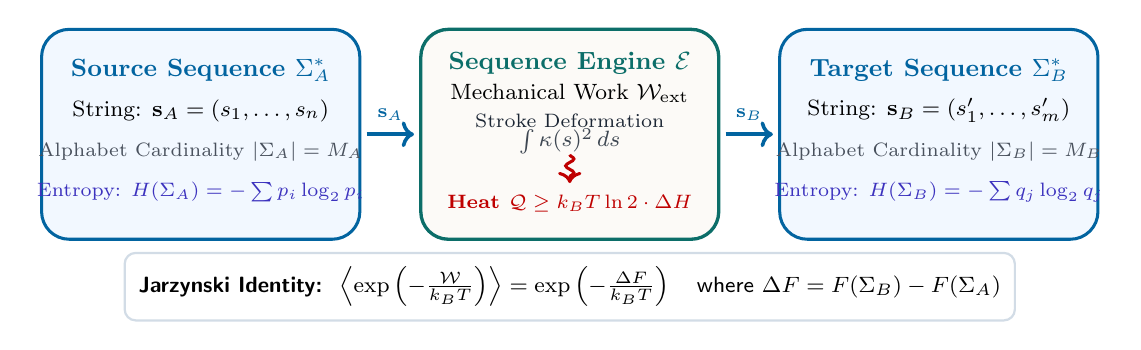
\begin{tikzpicture}[every node/.style={font=\small\sffamily}, scale=0.86]
    % Source Sequence Box
    \draw[fill=calloutbg, draw=primaryblue, line width=1.1pt, rounded corners=10pt] (-7.8,-1.55) rectangle (-3.1,1.55);
    \node[color=primaryblue, font=\bfseries\small] at (-5.45, 0.95) {Source Sequence $\Sigma_A^*$};
    \node[font=\footnotesize] at (-5.45, 0.35) {String: $\mathbf{s}_A = (s_1, \dots, s_n)$};
    \node[font=\scriptsize, color=darkslate!80] at (-5.45, -0.25) {Alphabet Cardinality $|\Sigma_A| = M_A$};
    \node[font=\scriptsize, color=accentindigo] at (-5.45, -0.85) {Entropy: $H(\Sigma_A) = -\sum p_i \log_2 p_i$};

    % Transformation Engine Middle Box
    \draw[fill=warmbg, draw=accentteal, line width=1.2pt, rounded corners=10pt] (-2.2,-1.55) rectangle (2.2,1.55);
    \node[color=accentteal, font=\bfseries\small] at (0, 1.05) {Sequence Engine $\mathcal{E}$};
    \node[font=\footnotesize] at (0, 0.60) {Mechanical Work $\mathcal{W}_{\text{ext}}$};
    \node[font=\scriptsize, color=darkslate] at (0, 0.20) {Stroke Deformation};
    \node[font=\footnotesize, color=darkslate!85] at (0, -0.10) {$\int \kappa(s)^2\,ds$};
    \draw[->, line width=1.1pt, color=red!75!black, decorate, decoration={snake, amplitude=1.5pt, segment length=5pt}] (0, -0.30) -- (0, -0.72);
    \node[font=\scriptsize\bfseries, color=red!75!black] at (0, -1.02) {Heat $\mathcal{Q} \ge k_B T \ln 2 \cdot \Delta H$};

    % Inter-box Arrows
    \draw[->, line width=1.3pt, color=primaryblue] (-3.0, 0.0) -- (-2.3, 0.0) node[midway, above=1pt, font=\scriptsize\bfseries] {$\mathbf{s}_A$};
    \draw[->, line width=1.3pt, color=primaryblue] (2.3, 0.0) -- (3.0, 0.0) node[midway, above=1pt, font=\scriptsize\bfseries] {$\mathbf{s}_B$};

    % Target Sequence Box
    \draw[fill=calloutbg, draw=primaryblue, line width=1.1pt, rounded corners=10pt] (3.1,-1.55) rectangle (7.8,1.55);
    \node[color=primaryblue, font=\bfseries\small] at (5.45, 0.95) {Target Sequence $\Sigma_B^*$};
    \node[font=\footnotesize] at (5.45, 0.35) {String: $\mathbf{s}_B = (s_1^\prime, \dots, s_m^\prime)$};
    \node[font=\scriptsize, color=darkslate!80] at (5.45, -0.25) {Alphabet Cardinality $|\Sigma_B| = M_B$};
    \node[font=\scriptsize, color=accentindigo] at (5.45, -0.85) {Entropy: $H(\Sigma_B) = -\sum q_j \log_2 q_j$};

    % Bottom Invariant Box
    \node[draw=boxborder, fill=white, rounded corners=4pt, line width=0.8pt, inner sep=5pt] at (0,-2.25) {
        \footnotesize\textbf{Jarzynski Identity:}\; $\left\langle \exp\left(-\frac{\mathcal{W}}{k_B T}\right) \right\rangle = \exp\left(-\frac{\Delta F}{k_B T}\right) \quad \text{where } \Delta F = F(\Sigma_B) - F(\Sigma_A)$
    };
\end{tikzpicture}
\caption{The Thermodynamic Cycle of Sequence Transformation: processing symbolic strings from alphabet $\Sigma_A$ to alphabet $\Sigma_B$ expends stroke curvature energy $\int \kappa(s)^2 ds$, performs work $\mathcal{W}$, and dissipates Landauer heat $\mathcal{Q}_{\text{diss}}$ into the physical substrate.}
\label{fig:thermodynamic_cycle}
\end{figure}

Topologically, character sets exhibit sharp variations in Euler characteristic $\chi = V - E + F$:
\begin{itemize}[noitemsep,topsep=1.5pt]
    \item \textbf{Genus 0 (Tree Glyphs):} Open curves with no enclosed counter-forms ($\chi = 1$), such as Latin \texttt{C, E, I, L, S, T, V, Z}. These require minimal ink-bleed correction and lowest rasterization energy.
    \item \textbf{Genus 1 (Monotoroidal Glyphs):} Single enclosed loop ($\chi = 0$), such as \texttt{A, D, O, P, R, Q}. In mechanical punch-cutting, these require internal counter-punches and high manufacturing pressure.
    \item \textbf{Genus 2 (Bitoroidal Glyphs):} Double enclosed loops ($\chi = -1$), such as \texttt{B} or \texttt{8}.
\end{itemize}

\subsection{Visual Classification Entropy and Perceptual Foveation}
When human readers or computer vision models inspect an orthographic text, the visual sensor executes rapid ballistic saccades followed by fixed foveations. The energetic cost of identifying a glyph $s \in \Sigma$ is bounded by the \textbf{perceptual classification entropy}:
\begin{equation}
\mathcal{H}_{\text{visual}}(\Sigma) = -\sum_{i=1}^{|\Sigma|} P(s_i) \log_2 P(s_i)
\end{equation}

\begin{table}[htbp]
\centering
\small
\begin{tabular}{lrrrr}
\toprule
\textbf{Writing System} & \textbf{Alphabet Size ($|\Sigma|$)} & \textbf{Entropy / Glyph} & \textbf{Mean Strokes} & \textbf{Topological Genus} \\
\midrule
Latin Alphabet & $26$ & $\sim 4.70\text{ bits}$ & $2.1\text{ strokes}$ & $0.35$ \\
Arabic Abjad & $28$ & $\sim 4.81\text{ bits}$ & $1.8\text{ strokes}$ & $0.28$ \\
Hangul Featural & $40$ & $\sim 5.32\text{ bits}$ & $3.4\text{ strokes}$ & $0.45$ \\
Ge'ez Abugida & $182$ & $\sim 7.51\text{ bits}$ & $3.8\text{ strokes}$ & $0.40$ \\
Hanzi Logographs & $3{,}500+$ & $\sim 11.77\text{ bits}$ & $9.2\text{ strokes}$ & $1.85$ \\
\bottomrule
\end{tabular}
\caption{Comparative Semiotic Typographic Physics: phonetic alphabets minimize per-glyph stroke work and topological complexity at the expense of longer sequence lengths, whereas logographic scripts maximize per-token informational payload at the cost of high mechanical stroke complexity.}
\label{tab:typographic_physics}
\end{table}

As formalized in Table~\ref{tab:typographic_physics}, human culture discovers a universal Pareto frontier balancing production and recognition work:
\begin{equation}
\mathcal{W}_{\text{total}} = \sum_{t=1}^N \Big( \mathcal{E}_{\text{stroke}}(s_t) + \lambda \mathcal{H}_{\text{visual}}(s_t) \Big)
\end{equation}
Logographic systems compress sequence length $N$ at the expense of high per-glyph stroke energy $\mathcal{E}(s)$. Phonetic alphabets expand string length $N$ while drastically reducing the manufacturing and classification cost per token.

\section{Algorithmic Information and String Transformations}

\subsection{Kolmogorov Complexity and Minimal Description}
Beyond physical ink, the informational content of a symbolic string $s \in \Sigma^*$ is measured by its \textbf{Kolmogorov complexity} $K_{\mathcal{U}}(s)$---the length of the shortest computer program $p$ running on a prefix-free universal Turing machine $\mathcal{U}$ that halts and outputs $s$:
\begin{equation}
K_{\mathcal{U}}(s) = \min_{p} \big\{ |p| : \mathcal{U}(p) = s \big\}
\end{equation}
In sequence translation $\tau: s_A \mapsto s_B$, the \textbf{conditional Kolmogorov complexity} $K(s_B \mid s_A)$ quantifies the irreducible computational program required to reconstruct the target string given the source text:
\begin{equation}
K(s_B \mid s_A) \le K(\tau) + \mathcal{O}(1)
\end{equation}
When translating between structurally isomorphic languages (e.g., Python to JavaScript or Italian to Spanish), $K(s_B \mid s_A)$ is small; the translation program $\tau$ exploits extensive shared grammatical regularities. When translating between distant representational regimes (e.g., vernacular poetic cadences to formal compiler intermediate representations), $K(s_B \mid s_A)$ approaches the full algorithmic entropy of the target sequence.

\subsection{Edit Distance as Thermodynamic Work}
In statistical string physics, converting source string $s_A$ into target string $s_B$ through atomic edit operations (insertions, deletions, substitutions) defines a trajectory through a discrete state space. Let $\mathcal{T} = (\sigma_0, \sigma_1, \dots, \sigma_T)$ be an editing trajectory where $\sigma_0 = s_A$ and $\sigma_T = s_B$.

The Levenshtein distance $d_L(s_A, s_B)$ corresponds to the \textbf{minimum mechanical action} along the optimal transformation path:
\begin{equation}
d_L(s_A, s_B) = \min_{\mathcal{T}} \sum_{t=1}^T c(\sigma_{t-1} \to \sigma_t)
\end{equation}
Under the \textbf{Jarzynski Equality} from non-equilibrium statistical mechanics, the average exponential work expended along stochastic editing trajectories matches the equilibrium free energy difference $\Delta F$:
\begin{equation}
\left\langle \exp\left(-\frac{\mathcal{W}_{\text{edit}}}{k_B T}\right) \right\rangle = \exp\left(-\frac{\Delta F}{k_B T}\right)
\end{equation}
where $\Delta F = F(s_B) - F(s_A)$ is the difference in algorithmic free energy. When editing strings out of equilibrium, the dissipated work $\mathcal{W}_{\text{diss}} = \langle \mathcal{W} \rangle - \Delta F \ge 0$ measures the thermodynamic inefficiency of the translation process.

\subsection{Tokenization Entropy and Vocabulary Cardinality}
In modern computational linguistics, text is segmented into subwords via algorithms such as Byte-Pair Encoding (BPE) or WordPiece. The choice of vocabulary size $|\mathcal{V}|$ represents a thermodynamic parameter governing memory bandwidth:
\begin{equation}
\mathcal{L}_{\text{seq}} = \frac{N_{\text{chars}}}{\bar{\ell}_{\text{token}}(|\mathcal{V}|)}, \quad H(\mathcal{V}) = \log_2 |\mathcal{V}|
\end{equation}
Expanding vocabulary size $|\mathcal{V}|$ shortens sequence length $\mathcal{L}_{\text{seq}}$, reducing quadratic attention computations $\mathcal{O}(\mathcal{L}^2)$ in Transformer architectures. However, it increases the parameter footprint of the embedding and unembedding matrices $W_{\text{emb}} \in \mathbb{R}^{|\mathcal{V}| \times d}$, increasing memory bus traffic. The optimal vocabulary size $|\mathcal{V}^*|$ minimizes the total energy expenditure across the memory hierarchy.

\section{The Physics of Machine and Human Learning}

\subsection{Free Energy Minimization in Sequence Processing}
Following the variational formulation of statistical physics (Jaynes, 1957; Friston, 2010), both biological cognitive circuits and deep sequence models process linguistic strings by minimizing a \textbf{Helmholtz Free Energy} functional $\mathcal{F}$:
\begin{equation}
\mathcal{F}(q, y) = \mathbb{E}_{q(\theta)}\big[ E(y, \theta) \big] - T \cdot S\big(q(\theta)\big)
\end{equation}
where $E(y, \theta) = -\ln p(y, \theta)$ is the internal energy (the cross-entropy sequence prediction loss), $S(q) = -\int q(\theta) \ln q(\theta) d\theta$ is the informational entropy of the parameter distribution, and $T$ is an effective cognitive or computational temperature.

Minimizing free energy enforces an optimal trade-off:
\begin{enumerate}[noitemsep,topsep=1.5pt]
    \item \textbf{Energy Minimization ($\mathbb{E}[E]$):} Maximizes accuracy in mapping source tokens to target sequences (adequacy).
    \item \textbf{Entropy Maximization ($-TS$):} Maximizes parameter dispersion and prevents brittle overfitting, ensuring robust generalization.
\end{enumerate}

\subsection{Langevin Dynamics and Thermal Gradient Noise}
During parameter optimization in neural machine translation models, gradient descent updates under stochastic gradient descent (SGD) follow discrete \textbf{overdamped Langevin diffusion}:
\begin{equation}
\frac{d\theta}{dt} = -\nabla \mathcal{L}(\theta) + \sqrt{\frac{2 k_B T_{\text{num}}}{\gamma}} \, \xi(t)
\end{equation}
where $\mathcal{L}(\theta)$ is the empirical sequence loss, $\xi(t)$ is Gaussian white noise satisfying $\langle \xi(t) \xi(t') \rangle = \delta(t - t')$, $\gamma$ is the numerical damping coefficient, and $T_{\text{num}} = \frac{\eta B_{\text{size}}}{2N}$ is the synthetic thermal temperature induced by mini-batch sampling noise with learning rate $\eta$.

Gradient descent is physically a process of heat dissipation: escaping shallow metastable saddle points requires thermal fluctuations proportional to $k_B T_{\text{num}}$, driving parameters toward the lowest free-energy attractor states on the loss surface.

\subsection{Memory Transport and Hardware Thermodynamic Costs}
In high-performance computational infrastructure, the thermodynamic cost of processing sequences is dominated not by arithmetic logic units (ALUs), but by \textbf{memory transport energy}:

\begin{table}[htbp]
\centering
\small
\begin{tabular}{lrr}
\toprule
\textbf{Hardware Operation} & \textbf{Energy Cost (pJ)} & \textbf{Relative Energy Multiplier} \\
\midrule
32-bit Floating Point Add / Multiply & $0.9\text{ pJ}$ & $1.0\times$ \\
SRAM On-Chip Cache Read (32-bit) & $5.0\text{ pJ}$ & $5.5\times$ \\
HBM / DRAM Off-Chip Fetch (32-bit) & $640.0\text{ pJ}$ & $711.1\times$ \\
Optical Board-to-Board Interconnect & $1{,}200.0\text{ pJ}$ & $1{,}333.3\times$ \\
\bottomrule
\end{tabular}
\caption{Microprocessor Energy Hierarchy: moving sequence representations across the physical memory wall consumes nearly three orders of magnitude more thermodynamic energy than executing arithmetic logic.}
\label{tab:memory_energy}
\end{table}

As Table~\ref{tab:memory_energy} proves, fetching symbolic tokens across the DRAM memory wall consumes $>700\times$ more energy than executing a mathematical operation. Therefore, typographic tokenization schemes (such as Byte-Pair Encoding or SentencePiece) are directly constrained by thermodynamics: compressing sequences into optimal token lengths minimizes physical memory fetches, directly minimizing power consumption in data centers.

\section{The Computational Laboratory}

The computational laboratory for this lecture implements physical stroke curvature evaluation and Landauer dissipation estimation for sequence transformations:

\begin{lstlisting}[language=Python, caption={Curvature energy and Landauer dissipation in sequence translation.}, label={lst:thermo}]
import numpy as np

def compute_stroke_curvature_energy(points: np.ndarray, alpha: float = 1.0, beta: float = 2.0) -> float:
    """
    Computes physical stroke bending energy:
        E = integral (alpha + beta * kappa^2) ds
    for a discretized glyph contour (N x 2).
    """
    # 1. Compute first-order differences (tangent arc length)
    dx = np.gradient(points[:, 0])
    dy = np.gradient(points[:, 1])
    ds = np.sqrt(dx**2 + dy**2) + 1e-8

    # 2. Compute second-order differences (curvature acceleration)
    ddx = np.gradient(dx)
    ddy = np.gradient(dy)
    
    # 3. Signed curvature kappa = |dx*ddy - dy*ddx| / (dx^2 + dy^2)^(3/2)
    curvature = np.abs(dx * ddy - dy * ddx) / (ds**3)
    energy = np.sum((alpha + beta * (curvature**2)) * ds)
    return float(energy)

def landauer_dissipation(entropy_erased_bits: float, temp_kelvin: float = 300.0) -> float:
    """
    Computes minimum theoretical thermodynamic dissipation:
        Q >= k_B * T * ln(2) * Delta_H (Joules)
    """
    k_B = 1.380649e-23  # Boltzmann constant in J/K
    q_min = k_B * temp_kelvin * np.log(2) * entropy_erased_bits
    return float(q_min)
\end{lstlisting}

\section{Seminar Discussion \& Socratic Prompts}

\socraticbox{Seminar Questions for Class Discussion}{%
\begin{enumerate}[noitemsep,topsep=1.5pt]
    \item \textbf{Thermodynamic Efficiency of Natural Alphabets:} Why did Phoenician, Greek, and Latin alphabets stabilize at roughly 20--30 phonetic symbols rather than expanding to 10,000 ideograms or collapsing to a 2-symbol binary alphabet? What thermodynamic trade-off between stroke manufacturing work and sequence length does this strike?
    \item \textbf{Reversible Computing and Lossless Translation:} If translation between two formal languages is a category-theoretic isomorphism ($F \circ G \cong \mathbf{1}$), can it theoretically be implemented on Bennett-style logically reversible hardware with zero Landauer dissipation?
    \item \textbf{The Energy Cost of Hallucination:} In large language models, generating divergent or hallucinated tokens increases sequence entropy. How does this entropy generation manifest in physical power draw across GPU clusters?
    \item \textbf{Typographic Wear and Historical Media:} How did the physical wear of lead type and mechanical punch-cutting historically constrain the evolution of European font designs (e.g., Blackletter vs. Antiqua)?
\end{enumerate}
}

\section{Laboratory Exercise}
For this week's laboratory assignment, clone and execute the companion computational notebook:
\begin{center}
    \texttt{notebooks/python/08\_thermodynamic\_semiotics.ipynb}
\end{center}

\textbf{Assignment Tasks:}
\begin{enumerate}[noitemsep,topsep=1.5pt]
    \item Vectorize TrueType glyph contours across three scripts (Latin, Arabic, and Hanzi) and calculate their mechanical stroke curvature energy $\mathcal{E}_{\text{stroke}}$.
    \item Measure empirical Landauer dissipation limits for token sequence translation across varying vocabulary compressions.
    \item Implement Langevin dynamic simulation on a 2D synthetic loss landscape to evaluate the role of thermal gradient noise in escaping non-convex saddle points.
\end{enumerate}

\subsection*{References}
\begin{enumerate}[label={[\arabic*]},noitemsep,topsep=1.5pt]
    \item Bennett, C. H. (1973). Logical reversibility of computation. \textit{IBM Journal of Research and Development}, 17(6), 525--532.
    \item Bringhurst, R. (1992). \textit{The Elements of Typographic Style}. Hartley \& Marks.
    \item Friston, K. (2010). The free-energy principle: a unified brain theory? \textit{Nature Reviews Neuroscience}, 11(2), 127--138.
    \item Jaynes, E. T. (1957). Information theory and statistical mechanics. \textit{Physical Review}, 106(4), 620--630.
    \item Kolmogorov, A. N. (1965). Three approaches to the quantitative definition of information. \textit{Problems of Information Transmission}, 1(1), 1--7.
    \item Landauer, R. (1961). Irreversibility and heat generation in the computing process. \textit{IBM Journal of Research and Development}, 5(3), 183--191.
    \item Shannon, C. E. (1948). A mathematical theory of communication. \textit{Bell System Technical Journal}, 27(3), 379--423.
\end{enumerate}

\vspace{0.3em}
\hrule height 0.4pt \vspace{0.3em}
\noindent{\scriptsize\sffamily\color{darkslate!70} Semantic Mechanics Project $\cdot$ Mathematical Linguistics Group}

\end{document}
